\documentclass{article}
	\usepackage{geometry}
	\geometry{left=2cm,right=2cm}
	\usepackage{graphicx}
	\usepackage{indentfirst}
	\usepackage[hyphens]{url}
	\usepackage{listings}
	\usepackage{color}
	\definecolor{gray}{rgb}{0.3,0.3,0.3}
	\usepackage{caption}
	\DeclareCaptionFont{white}{\color{white}}
	\DeclareCaptionFormat{listing}{\colorbox{gray}{\parbox{\textwidth}{#1#2#3}}}
	\captionsetup[lstlisting]{format=listing,labelfont={bf,sf,white},textfont={bf,sf,white}}
	\usepackage{xcolor}
	\usepackage{booktabs}
	\captionsetup[table]{labelfont=bf}
	\usepackage[colorlinks,linkcolor=red]{hyperref}

	\begin{document}
		\begin{center}\textbf{Bo Zhang\\01063214}
		\end{center}
		\section{Create a blog-term matrix}
		Create a blog-term matrix. Start by grabbing 100 blogs; include:\\
		\indent\url{http://f-measure.blogspot.com/}\\
		\indent\url{http://ws-dl.blogspot.com/}\\
		and grab 98 more as per the method shown in class.\\
		\indent Use the blog title as the identifier for each blog. Use the terms from every item/title (RSS) or entry/title (Atom) for the columns of the matrix. The values are the frequency of occurrence. Essentially you are replicating the format of the ``blogdata.txt'' file included with the PCI book code. Limit the number of terms to the most ``popular'' 1000 terms, this is *after* the criteria on p. 32 (slide 7) has been satisfied. Remember that blogs are paginated.\\

		\noindent\textbf{Algorithm: }\\
		\indent1. Open the URL of ``Next Blog'' 500 times to get 500 Blog URLs.\\
		\indent2. For each time opening the URL, get a BeautifulSoup object, extract the Atom link, save it to \href{https://github.com/zhangboroy/cs532-s17/blob/master/assg08_submission/feedlist.txt}{``feedlist.txt''} and open it.\\
		\indent3. Get a BeautifulSoup object with the new page, extract the link of ``Next Page''(if any), save it to \href{https://github.com/zhangboroy/cs532-s17/blob/master/assg08_submission/feedlist.txt}{``feedlist.txt''} and open it.\\
		\indent4. Repeat Step 3 again and again until there is no ``Next Page''.\\
		\indent5. Open the URLs of Blog ``f-measure'' and ``ws-dl'', finish the Steps 2-4 of each Blog but use \href{https://github.com/zhangboroy/cs532-s17/blob/master/assg08_submission/feedlistReady.txt}{``feedlistReady.txt''} as the output file.\\
		\indent6. Open \href{https://github.com/zhangboroy/cs532-s17/blob/master/assg08_submission/feedlist.txt}{``feedlist.txt''} to read all the URLs to a list.\\
		\indent7. Use ``set'' method to remove duplicated URLs.\\
		\indent8. Open the remaining URLs 1 by 1, use the Blog title and the package \href{https://pypi.python.org/pypi/langid}{``langid''} to remove non-English Blogs.\\
		\indent9. Save the first 98 remaining URLs to \href{https://github.com/zhangboroy/cs532-s17/blob/master/assg08_submission/feedlistReady.txt}{``feedlistReady.txt''} and the others to \href{https://github.com/zhangboroy/cs532-s17/blob/master/assg08_submission/feedlistMore.txt}{``feedlistMore.txt''}.\\
		\indent10. Use the script from ``Programming Collective Intelligence'' to open \href{https://github.com/zhangboroy/cs532-s17/blob/master/assg08_submission/feedlistReady.txt}{``feedlistReady.txt''} and count all the words from the 100 Blogs.\\
		\indent11. Edit the script to add the frequency to the word list and sort the word list by frequency.\\
		\indent12. Generate the blogdata with top 1000 words in the word list and save it as \href{https://github.com/zhangboroy/cs532-s17/blob/master/assg08_submission/blogdata(allFilter).txt}{``blogdata(allFilter).txt''}.\\

		\noindent\textbf{Source code:}
		\lstinputlisting[language=python, breakatwhitespace=false, label=BlogURLdownload.py, caption=The content of BlogURLdownload.py]{BlogURLdownload.py}

		\noindent\\\textbf{Results:}\\
		\indent\href{https://github.com/zhangboroy/cs532-s17/blob/master/assg08_submission/feedlist.txt}{feedlist.txt}\\
		\indent\href{https://github.com/zhangboroy/cs532-s17/blob/master/assg08_submission/feedlistReady.txt}{feedlistReady.txt}\\
		\indent\href{https://github.com/zhangboroy/cs532-s17/blob/master/assg08_submission/feedlistMore.txt}{feedlistMore.txt}\\
		\indent\href{https://github.com/zhangboroy/cs532-s17/blob/master/assg08_submission/blogdata(allFilter).txt}{blogdata(allFilter).txt}\\

		\section{Hierarchical Clustering}
		Create an ASCII and JPEG dendrogram that clusters the most similar blogs. Include the JPEG in your report and upload the ascii file to github.\\

		\noindent\textbf{Algorithm:}\\
		\indent1. Use the script from ``Programming Collective Intelligence'' to open \href{https://github.com/zhangboroy/cs532-s17/blob/master/assg08_submission/blogdata(allFilter).txt}{``blogdata(allFilter).txt''}.\\
		\indent2. Run the Hierarchical Clustering.\\
		\indent3. Save the ASCII dendrogram to \href{https://github.com/zhangboroy/cs532-s17/blob/master/assg08_submission/ASCII%20dendrogram(Q2).txt}{``ASCII dendrogram(Q2).txt''}.\\
		\indent4. Save the JPEG dendrogram to \href{https://github.com/zhangboroy/cs532-s17/blob/master/assg08_submission/blogclust(Q2).jpg}{``blogclust(Q2).jpg''}.\\

		\noindent\textbf{Source code:}
		\lstinputlisting[language=python, breakatwhitespace=false, label=Q2.py, caption=The content of Q2.py]{Q2.py}

		\noindent\\\textbf{Results:}\\
		\indent\href{https://github.com/zhangboroy/cs532-s17/blob/master/assg08_submission/ASCII%20dendrogram(Q2).txt}{ASCII dendrogram(Q2).txt}\\
		\begin{figure}[!htb]
			\centering 
			\href{https://github.com/zhangboroy/cs532-s17/blob/master/assg08_submission/blogclust(Q2).jpg}
			{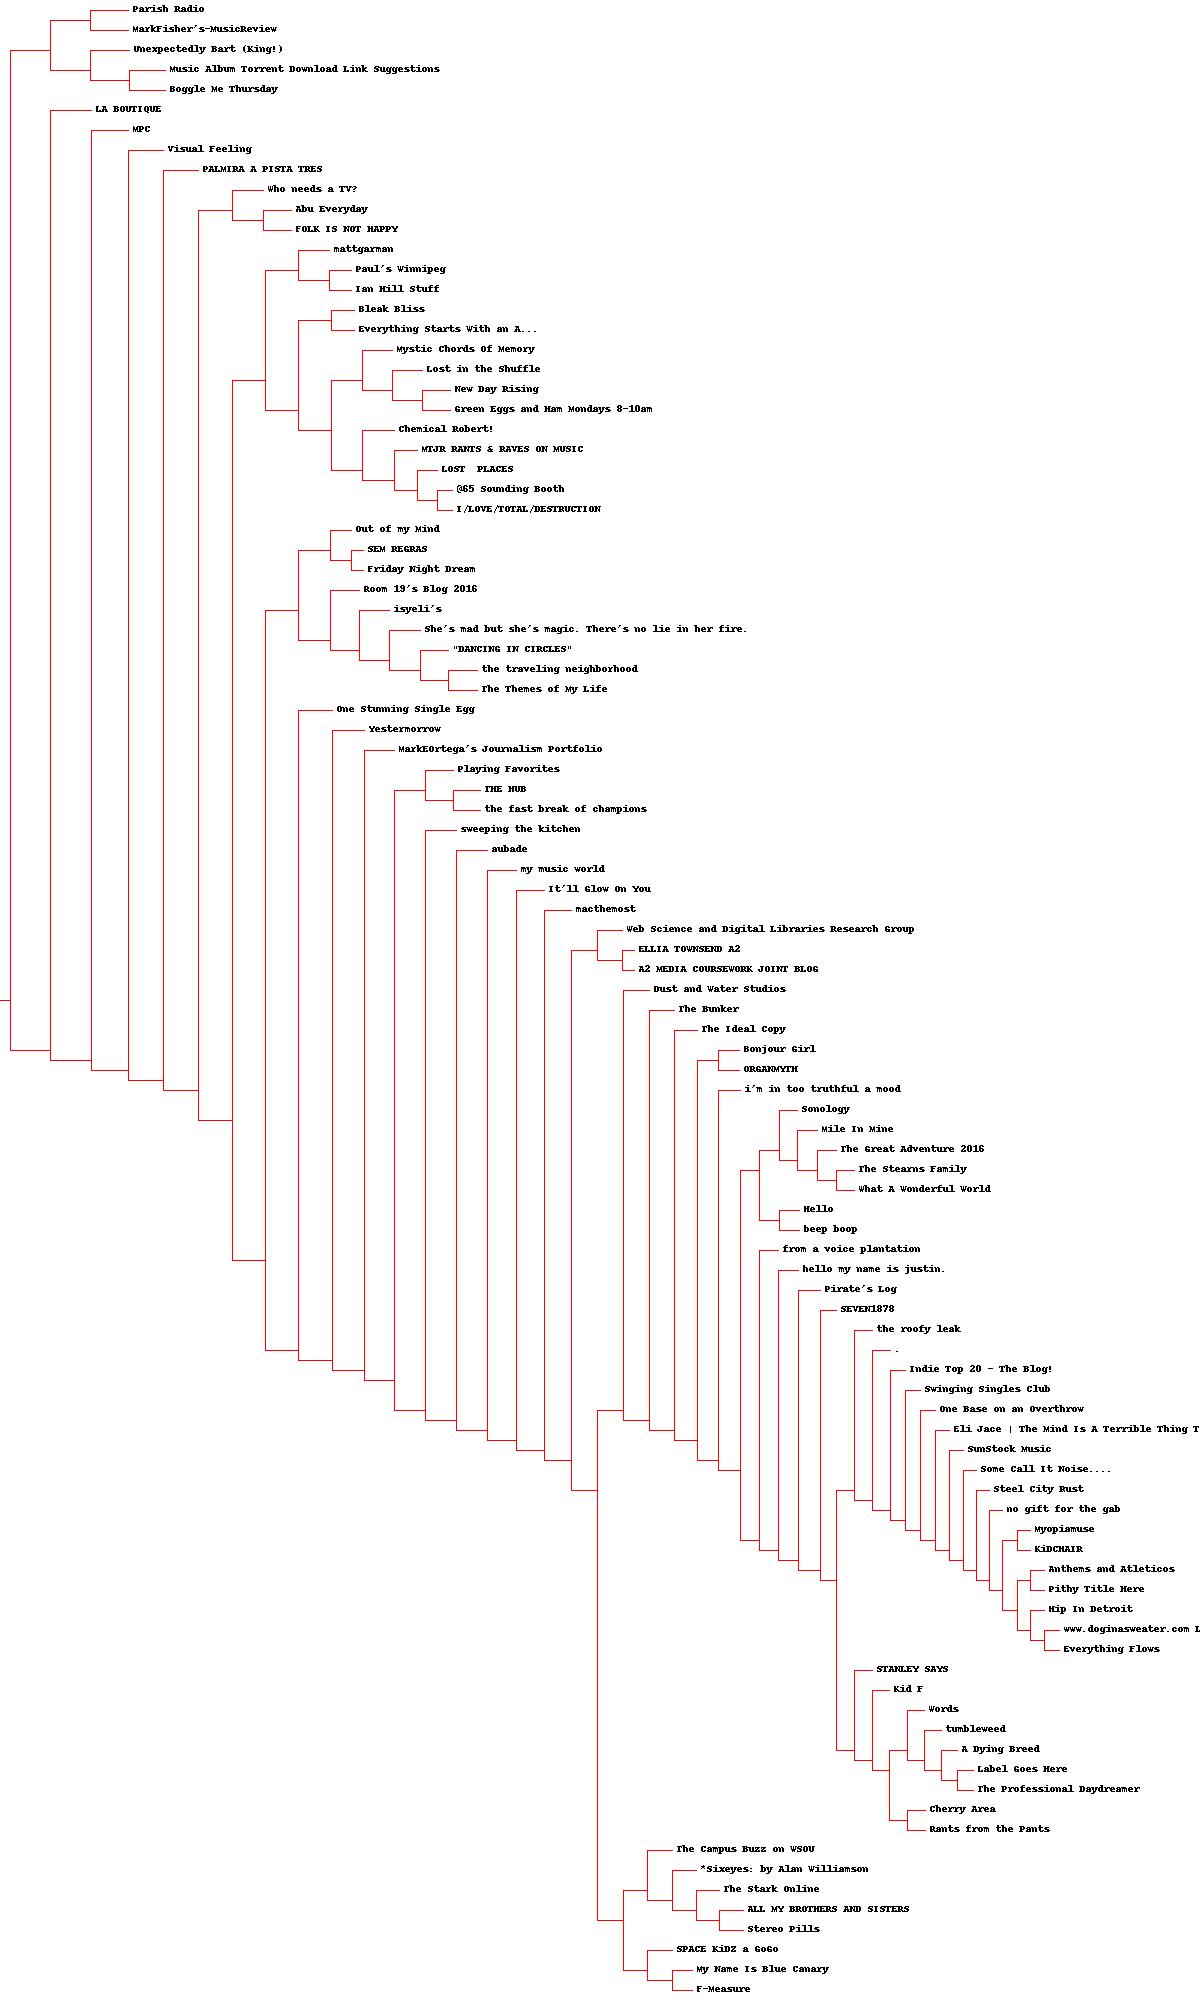
\includegraphics[width=0.3\textwidth]{blogclust(Q2).jpg}}
			\label{fig:blogclust(Q2)}
			\caption{blogclust(Q2)}
		\end{figure}

		\section{K-Means Clustering}
		Cluster the blogs using K-Means, using k=5,10,20. Print the values in each centroid, for each value of k. How many interations were required for each value of k?\\

		\noindent\textbf{Algorithm:}\\
		\indent1. Use the script from ``Programming Collective Intelligence'' to open \href{https://github.com/zhangboroy/cs532-s17/blob/master/assg08_submission/blogdata(allFilter).txt}{``blogdata(allFilter).txt''}.\\
		\indent2. Run the K-Means Clustering with k=5,10,20.\\
		\indent3. Print all the centroid.\\

		\noindent\textbf{Source code:}
		\lstinputlisting[language=python, breakatwhitespace=false, label=Q3.py, caption=The content of Q3.py]{Q3.py}

		\noindent\\\textbf{Results: }\href{https://github.com/zhangboroy/cs532-s17/blob/master/assg08_submission/K-Means.txt}{K-Means.txt}\\
		\section{Multidimensional Scaling}
		Use MDS to create a JPEG of the blogs similar to slide 29 of the week 12 lecture. How many iterations were required?\\

		\noindent\textbf{Algorithm:}\\
		\indent1. Use the script from ``Programming Collective Intelligence'' to open \href{https://github.com/zhangboroy/cs532-s17/blob/master/assg08_submission/blogdata(allFilter).txt}{``blogdata(allFilter).txt''}.\\
		\indent2. Edit the ``scaledown'' function to make output both step number and error.\\
		\indent3. Do the Multidimensional Scaling and draw the two-dimensional chart as \href{https://github.com/zhangboroy/cs532-s17/blob/master/assg08_submission/blogs2d.jpg}{``blogs2d.jpg''}.\\

		\noindent\textbf{Source code:}
		\lstinputlisting[language=python, breakatwhitespace=false, label=Q4.py, caption=The content of Q4.py]{Q4.py}

		\noindent\\\textbf{Results: }Total iterations are 255(\href{https://github.com/zhangboroy/cs532-s17/blob/master/assg08_submission/Q4.txt}{Q4.txt})\\
		\begin{figure}[!htb]
			\centering 
			\href{https://github.com/zhangboroy/cs532-s17/blob/master/assg08_submission/blogs2d.jpg}
			{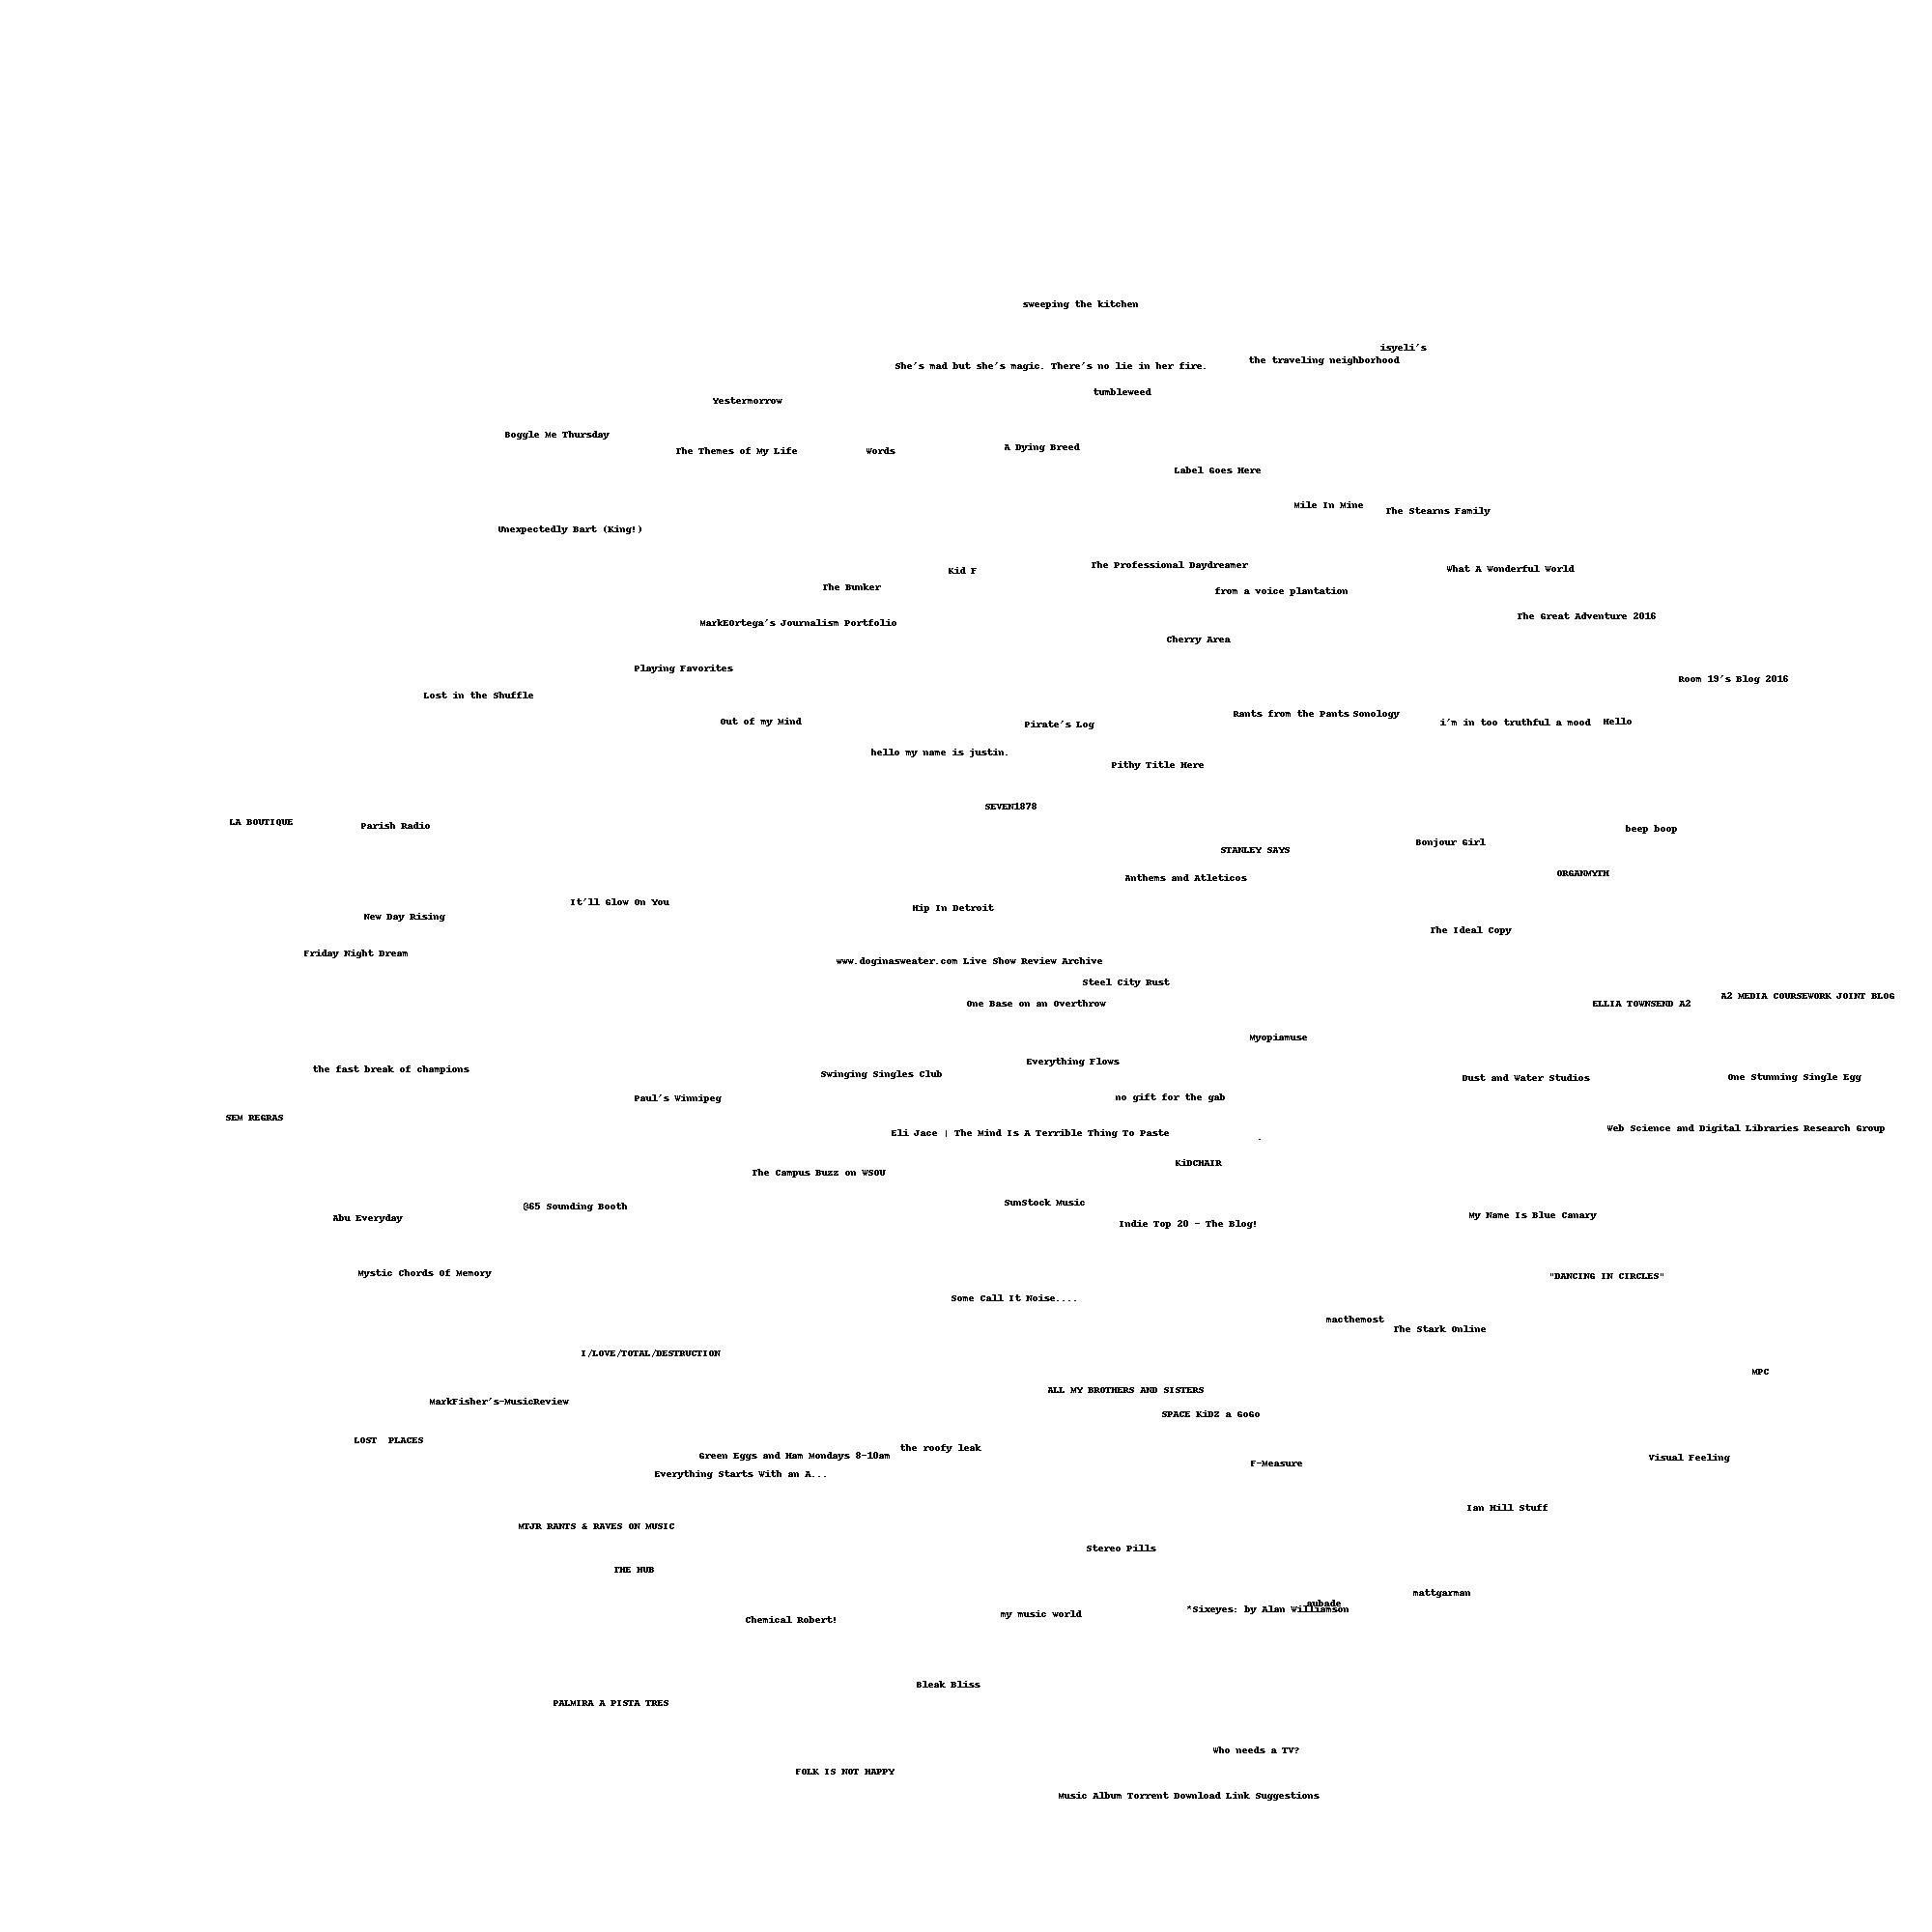
\includegraphics[width=0.79\textwidth]{blogs2d.jpg}}
			\label{fig:blogs2d}
			\caption{blogs2d}
		\end{figure}
		\section{TFIDF}
		Re-run question 2, but this time with proper TFIDF calculations instead of the hack discussed on slide 7 (p. 32). Use the same 1000 words, but this time replace their frequency count with TFIDF scores as computed in assignment \#3. Document the code, techniques, methods, etc. used to generate these TFIDF values. Upload the new data file to github.\\
		\indent Compare and contrast the resulting dendrogram with the dendrogram from question \#2.\\

		\noindent\textbf{Algorithm:}\\
		\indent1. Use the script from ``Programming Collective Intelligence'' to open \href{https://github.com/zhangboroy/cs532-s17/blob/master/assg08_submission/blogdata(allFilter).txt}{``blogdata(allFilter).txt''}.\\
		\indent2. Compute the TFIDF of each term of each Blog and save them to \href{https://github.com/zhangboroy/cs532-s17/blob/master/assg08_submission/blogdata(Q5).txt}{``blogdata(Q5).txt''}.\\
		\indent3. Run the Hierarchical Clustering.\\
		\indent4. Save the ASCII dendrogram to \href{https://github.com/zhangboroy/cs532-s17/blob/master/assg08_submission/ASCII%20dendrogram(Q5).txt}{``ASCII dendrogram(Q5).txt''}.\\
		\indent5. Save the JPEG dendrogram to \href{https://github.com/zhangboroy/cs532-s17/blob/master/assg08_submission/blogclust(Q5).jpg}{``blogclust(Q5).jpg''}.\\

		\noindent\textbf{Source code:}
		\lstinputlisting[language=python, breakatwhitespace=false, label=TFIDF.py, caption=The content of TFIDF.py]{TFIDF.py}
		\lstinputlisting[language=python, breakatwhitespace=false, label=Q5.py, caption=The content of Q5.py]{Q5.py}

		\noindent\\\textbf{Results:}\\
		\indent\href{https://github.com/zhangboroy/cs532-s17/blob/master/assg08_submission/ASCII%20dendrogram(Q5).txt}{ASCII dendrogram(Q5).txt}\\
		\begin{figure}[!htb]
			\centering 
			\href{https://github.com/zhangboroy/cs532-s17/blob/master/assg08_submission/blogclust(Q5).jpg}
			{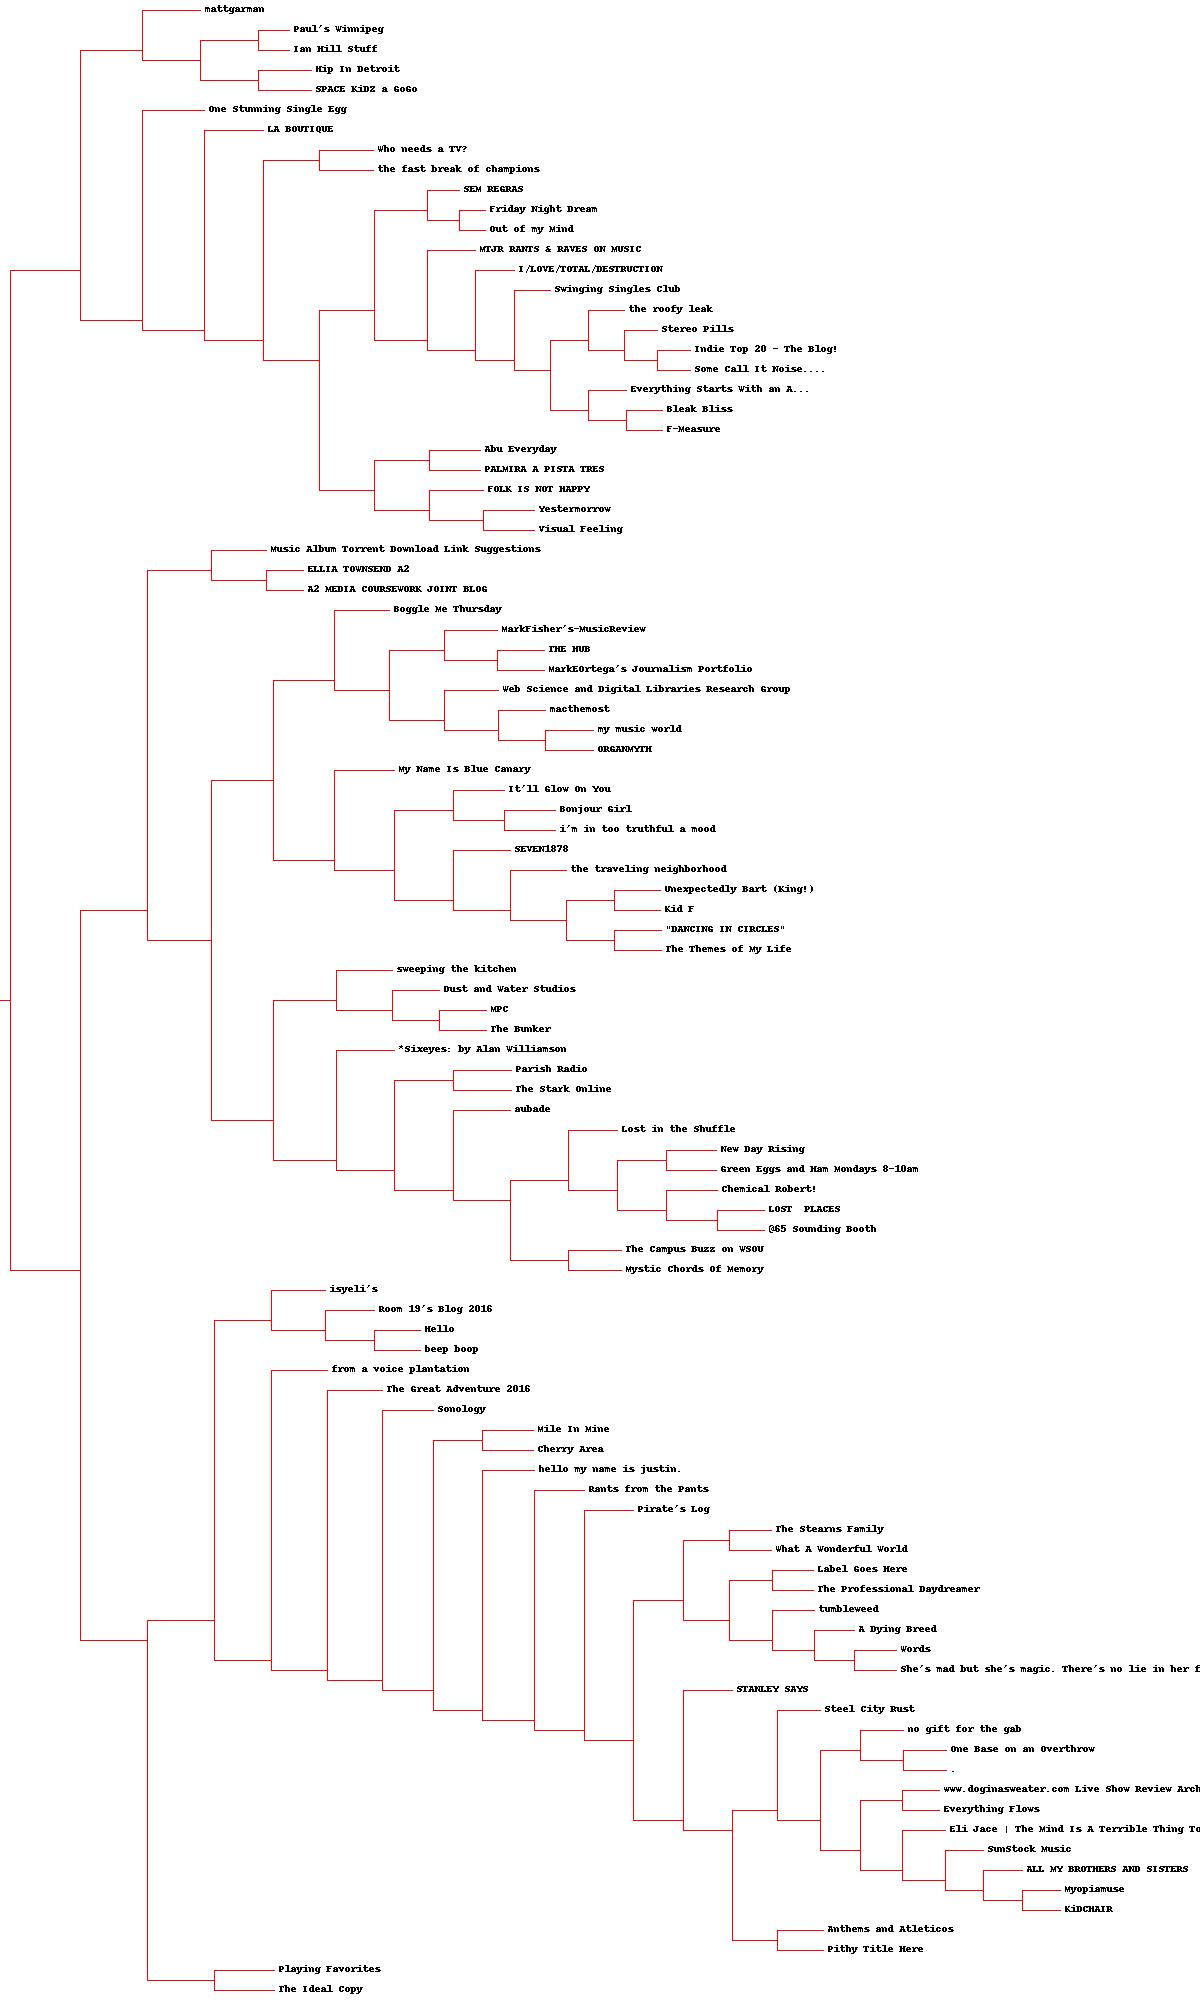
\includegraphics[width=0.33\textwidth]{blogclust(Q5).jpg}}
			\label{fig:blogclust(Q5)}
			\caption{blogclust(Q5)}
		\end{figure}

		According to the result from Q2, if we split all Blogs into 2 groups, there are only 5 Blogs in the top group. According to the result from Q5, if we do the same split, there are 27 groups in the top group. The split seems more balanced with this method.\\
	\end{document}